\chapter{Problem Statement and our Remarks}
%
% A glimpse on what set of variables are NOT independent, or NOT DEFINITELY independent. (Maybe this goes to the proof section)
%
\epigraph{Nobody can give you freedom. Nobody can give you equality or justice or anything. If you're a man, you take it.}{\textit{Malcolm X}}
%
\section{Introduction}
In order to prove that a function is \hyperref[sec:memory-hard]{\emph{memory-hard}} (see \hyperref[sec:memory-hard]{section}~\ref{sec:memory-hard}) we need to show that no implementation exists, that can produce the same result using less memory without significant time cost. In other words, using an implementation which needs less memory is not something that can give advantage to some miner because the time factor will make the procedure equally or more \emph{expensive}, even if the miner uses parallel computation techniques. Reproduced from CryptoNote~\cite{cryptonight}:
\begin{verbatim}
  CryptoNight is a memory-hard hash function. It is designed to be
  inefficiently computable on GPU, FPGA and ASIC architectures.
\end{verbatim}

In Monero mining, CPU's cores are only efficient if they can use the super fast 2MB cache over and over. Each core needs about 2MB for CryptoNight to stay cached. So a miner should check how much L2 cache or - in rare cases - also L3 cache the CPU has. Then divide by 2MB and this will be how many cores he/she can run at the same time.

There are several reasons to suspect that CryptoNight could be a memory-hard function. One of the most popular arguments was that a megabyte of internal memory is an almost unacceptable size for a modern ASIC pipeline. But hardware is constantly evolving and eventually there was recently an effort for Monero ASIC production. The first documented effort was the ASIC called \emph{Antminer X3} by Bitmain~\cite{bitmain}. The announcement was made in March 2018. Observing the raise of hashrate in the network, it was obvious that there were ASICs used for mining.

Founded in 2013, Bitmain, is a firm that produces ASIC chips and mines Bitcoin. The firm also operates \emph{Antpool}, which according to observers is the largest Bitcoin mining pool. An ASIC device by Bitmain has been mining Bitcoins for many years.

The reason Monero is planning to make Bitman’s Antminer X3 ineffective, is that it could enable some forms of attacks. These attacks could result in the mining pool taking over principal cryptocurrency’s hashrate. The act may enable double spending of coins, false transaction histories and censoring payments.

Riccardo Spagni, in a response to a Twitter comment which sees ASICs as a good thing~\cite{fluffypony}, said:
\begin{verbatim}
  Removing all of the hashrate distributed among tens of
  thousands of miners, in favour of a handful of miners
  that can afford an overpriced machine from a single
  manufacturer is GOOD for security?
  I doubt even you believe that.
\end{verbatim}

There were some thoughts like "\emph{How did they do this? Isn't CryptoNight memory-bound?}". Well, one thing is that CryptoNight is \emph{ASIC-resistant}, not \emph{ASIC-proof}\footnote{ASIC manufacturers are discouraged from building an ASIC for Monero mining, but there is no formal mathematical proof stating that an ASIC cannot be built.}. But, that was not the problem. Another thought is that L3 cache supports a lot of extra functionality like being shared across cores, writing back to RAM, being behind two other levels of cache, etc. which all makes it a lot less efficient (among other issues with the approach). But, again, that was not the case in that particular effort.

L3 latency wasn't the issue. ASICs just traded latency for bandwidth the same way GPUs do. They were built on stacks of DRAM, not lightning fast caches. The costs of cache complexity aren't only latency but also power usage and die space. Raw speed isn't even necessarily the goal for either CPUs or GPUs or ASICs here, it is efficiency.

But Monero project reacted and announced upgrades bi-annually in order to keep ASICs at bay. Upgrades are a problem, because upgrades produce bugs and vulnerabilities. Especially when they are that frequent. On the other hand, upgrades in Monero are minor, with no changes in the memory-hard part. From this experience, we understand that a formal proof, or even a better understanding of the memory-hardness property in practice, is vital for its mining function in order to protect a cryptocurrency from centralization.

\section{Proof approach}
Our starting plan was quite simple. The moment we understood the operations that took place in the computation, we had a specific strategy in mind. We would prove:

First case (\emph{honest} miner):
\begin{itemize}
  \item If the input is uniformly at random chosen, then the output is of the same nature \textbf{AND} independent from the input. (one round)
  \item The above expands to the whole function, not just one round.
\end{itemize}

What we wanted to show, with the two steps above, is the following: No shortcuts exist for the calculations involved. If the miner is honest, then the hash of the block will be uniformly at random chosen and so will be the elements of the input ($a$, $b$ and $SP$) of the second stage. If that implies that the output of this process is also chosen uniformly at random, then every operation on the input cannot be guessed except with negligible probability, ergo no shortcut of this process exists.

Of course, another requirement is the input ($a,b,SP$) to be independent from the output ($a',b',SP'$), where $SP'$ is the modified $SP$ after the round. If this is not the case, then there is a relation between two or more elements and in the nature of that relation a chance for an attack may hide.

It is easy to expand the above hypothetical result to the function as a whole. Every round produces a uniformly at random chosen result. Thus, the last round will produce a uniformly at random distributed result too.

Second case (\emph{malicious} miner):
\begin{itemize}
  \item If the input is \textbf{NOT} chosen at random, then the output is \textbf{STILL} uniformly at random chosen \textbf{AND} independent from the input. (one round)
  \item The above expands to the whole function, not just one round.
\end{itemize}

If we had the results for the honest case, then the next step would be to show that even if the miner is malicious he cannot do any better for himself. Even if the input is not chosen uniformly at random, the result will be distributed uniformly. That means that even if we "fixed" the input to our taste, we could not guess the result except with negligible probability. The second step follows a similar train of thought as in the case of the honest miner.

If we managed to prove the above, that would be a proof of the CryptoNight's memory-hardness property. If we cannot find a shortcut for the process, then we cannot find a way to calculate the result with less memory or less time. Let us elaborate on the details of our research.

\subsection{The model}
Based on the aforementioned plan and with help from the observations and assumptions we made in \hyperref[sec:analysis]{section}~\ref{sec:analysis}, we now present the model of computation we assume for CryptoNight's second stage (see \hyperref[fig:model]{figure}~\ref{fig:model}).

The reader can see that there is a natural division of the process in three parts. The first part is the set of all operations performed on the first address' value. Explicitly, that involves:
\begin{description}
  \item [Read] Input to an AES operation. Under our assumption, AES is a pseudorandom function (PRF).
  \item [Write] The result of a XOR ($\oplus$) operation.
\end{description}

The second part involves any operation performed on the second address' value. More precisely:
\begin{description}
  \item [Read] Store the value of the address.
  \item [Write] The result of a multiplication and an addition.
\end{description}

The third part is not of much interest for our purposes. It extracts the two outputs needed as input for next round of the second stage:
\begin{itemize}
  \item A XOR ($\oplus$) operation on the result of the addition that produces the first input of the next round ($a'$).
  \item The result of the PRF operation (AES) that is passed as the second input of the next round ($b'$).
\end{itemize}
\clearpage
%% natwidth=210mm, natheight=297mm :: A4 sizes

\begin{figure}[H]
  \centering
  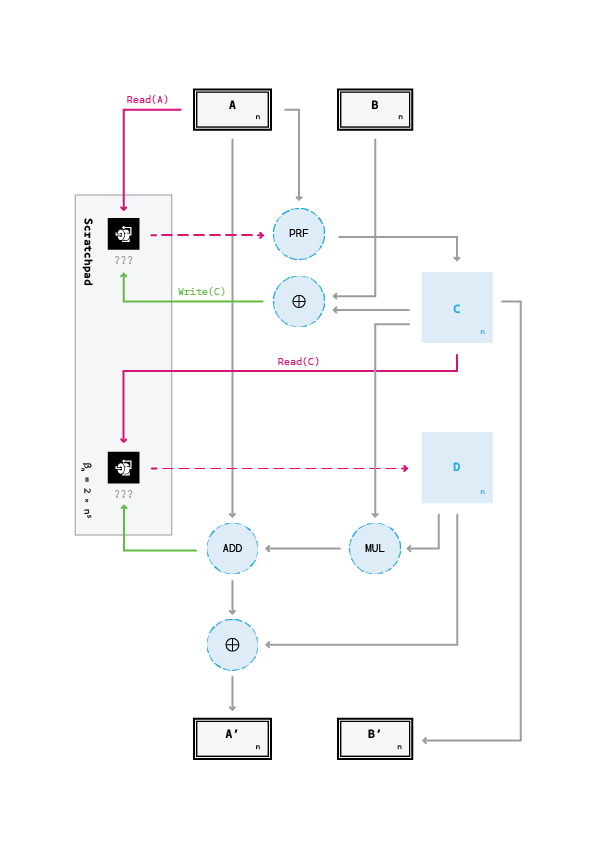
\includegraphics[scale=0.55, keepaspectratio]{Images/Bill/model.png}
  \caption{The model.~\cite{bill}}
  \label{fig:model}
\end{figure}

Here we note again (see \hyperref[sec:operations]{section}~\ref{sec:operations}) the special nature of the multiplication. Just for our purposes, we assume that it sustains the properties of its input. If the input (the two integers, each of size $n$) is uniformly at random chosen then the output of the multiplication is of the same nature. We strongly declare that this is \textbf{NOT} the case for the specific implementation of this operation. However, we will see that even with this assumption, we will not achieve our goal.

\subsection{The road to proof construction}
Based on the above we begin our analysis. Under the following assumptions,
\begin{itemize}
  \item $a,b$ are uniformly at random chosen
  \item AES is a PRF
\end{itemize}
we get that the first address of the round is changed in a way that does not change the distribution of the scratchpad. Everything seems fine.

For the second address we get the same result. Our assumptions are:
\begin{itemize}
  \item AES is a PRF
  \item $\forall c : SP_c$ is uniformly at random chosen
  \item Multiplication and addition sustain the distribution of their inputs
\end{itemize}

Let's see the values of $a'$ and $b'$:
\begin{align} \label{eq:normal_1}
  a' &= \Big( a + \big( PRF(a, SP_{a}) \cdot SP_{PRF(a, SP_a)} \big) \Big) \oplus SP_{PRF(a, SP_a)}\\ b' &= PRF(a, SP_{a}) \label{eq:normal_2}
\end{align}

Here we have a major problem. The problem is not the distribution of the output. Under our assumptions that is appropriate. But,
\begin{itemize}
  \item $a'$ is \textbf{NOT} independent from $a$
  \item $b'$ is \textbf{NOT} independent from $b$
  \item $SP'$ (scratchpad after the round) is not uniformly at random chosen
\end{itemize}
The third statement comes out of the observation that the value of $SP_a$, after the write operation, is dependent on the value of $b$. These are observations that spoil our plan.

However, this is a hint to the possibility of the existence of a successful attack on the memory-hardness property of CryptoNight function. Part of the input of this stage (values of $a,b$) is produced right from the hashed input of CryptoNight (see \hyperref[sec:first]{sections}~\ref{sec:first},~\ref{sec:second}). If someone can control the value of $a$, or maybe some bits of $a$, then he has a partial control of the value of $a'$ or at least some control over the range of $a'$. The same apply to the values of $b$ and $b'$.

This is, of course, nothing more than an intuition, so let's see if we can achieve the planning of said attack.
%% Trying the attack approach
\section{Attack approach}
The above intuition, apart from the assumptions involved, implies a level of control over the value of $a$ or $b$ or both. This can be done with grinding techniques. In a very high level of abstraction, the miner can hash the input multiple times with Keccak, changing every time something in the block (nonce, sequence of transactions, etc.). That will give him a different digest every time, ergo a different value for $a$ and $b$. This is quite efficient, especially if an ASIC is involved.

But we will make a stronger assumption. We will assume that some adversarial miner has a total control over the value of $a$ and $b$. We will show that even in that case, an attack seems impossible. Due to the nature of our results, it doesn't make sense to analyze the way an attacker can gain control over the value of $a$ or $b$.

\subsection{What can we do?}
What is the level of impact that we can cause, if we could control the values of $a$ and $b$? What is the best we can do in order to achieve our goal?

If someone takes his/her time observing the process, he/she can see the only thing that we can hope for. That is to find an address $a$, with a content $SP_a$ such that:
\begin{equation} \nonumber
  \mbox{AES}(a,SP_a) = a
\end{equation}

The reader can see the visualization of this scenario in \hyperref[fig:attack]{figure}~\ref{fig:attack}. Now it is time to measure the probability of this event. If this probability is negligible, we cannot find anything more that we can do. We have $\beta_n$ addresses on the scratchpad and in the CryptoNight description~\cite{cryptonight} we see that:
\begin{verbatim}
  When a 16-byte value needs to be converted into an address in
  the scratchpad, it is interpreted as a little-endian integer,
  and the 21 low-order bits are used as a byte index. However,
  the 4 low-order bits of the index are cleared to ensure the
  16-byte alignment.
\end{verbatim}

This means that, for a uniformly at random chosen 16-byte number, the probability for the value to be converted into a specific address in the scratchpad is:
\begin{equation} \nonumber
  \frac{1 \cdot \mbox{\textbf{sizeof}}(\mbox{address})}{\mbox{\textbf{sizeof}}(SP)} =
  \frac{1 \cdot n}{\beta_n} = \frac{n}{2 \cdot n^5} = \frac{1}{2 \cdot n^4} = \frac{1}{\mbox{\textbf{poly}}(n)}
\end{equation}

That is, for all intents and purposes, \textbf{NOT} a negligible probability with respect to the size of $n$. Hence, that is something that we can do efficiently enough. Let's see what this scenario gives us, as a round outcome. If the reader cares to do some math, he/she will see that \hyperref[eq:normal_1]{equations}~\ref{eq:normal_1},~\ref{eq:normal_2} become:
\begin{align} \nonumber
  a' &= \Big( a + \big( a \cdot (a \oplus b) \big) \Big) \oplus (a \oplus b) &
  &\mbox{and} & b' &= a
\end{align}

This looks really promising. Until we see what happens to the next round. The one thing that the reader is suggested to observe is that, although $a'$ is a function of $a$ and $b$, it is certainly not equal to either of them.

In the next round, the value $a'$ will point to a different location on the scratchpad ($SP_{a'}$) and the value $\mbox{PRF}(a', SP_{a'})$ will point to a random address in the scratchpad. And this is exactly the moment we lose the control we had over the process.
\clearpage

\begin{figure}[H]
  \centering
  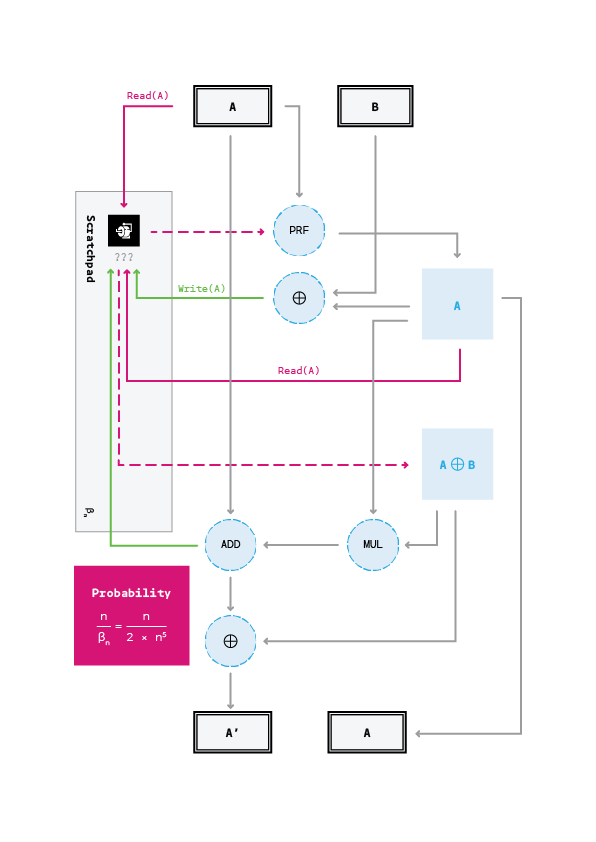
\includegraphics[scale=0.65, keepaspectratio]{Images/Bill/attack.png}
  \caption{The attack scenario.~\cite{bill}}
  \label{fig:attack}
\end{figure}
